In this Chapter, we detail methodology used for optimal sizing of stand-alone solar PV systems, more specifically using model checking. Diagrams, flowcharts, and algorithms support and explain the solutions.

In addition, we present all the underlying assumptions and premises. We also present the case studies used to evaluate the proposed approach for optimal sizing of stand-alone solar PV systems using automated synthesis. Moreover, the approach is compared with the HOME Pro simulation tool. The version and command-line of each verifier, the computing setup, the objectives of the experimental phase, and the results are also described.

It is important to emphasize that the complete explanation of the theoretical basis of the subject discussed here is presented in the Chapter~\nameref{chap:background}. In addition, knowledge of the literature is essential to aid understanding.

\section{Methodology for Optimal Sizing of Solar PV Systems}

Fig.~\ref{fig:optimization} illustrates how to obtain optimal sizing of a stand-alone solar PV system, beginning with the traditional techniques (manual, and simulation), and moving on to the proposed automatic synthesis detailed in this Section. 

Once more, as described in the automated verification process, the input information is the same for all the methods, with the difference that in automated validation it is possible to define the bound $k$ to restrict the design-space search. And the outputs are not equal, as in the design-space coverage and, mainly, in the final result.

\begin{figure}[h]
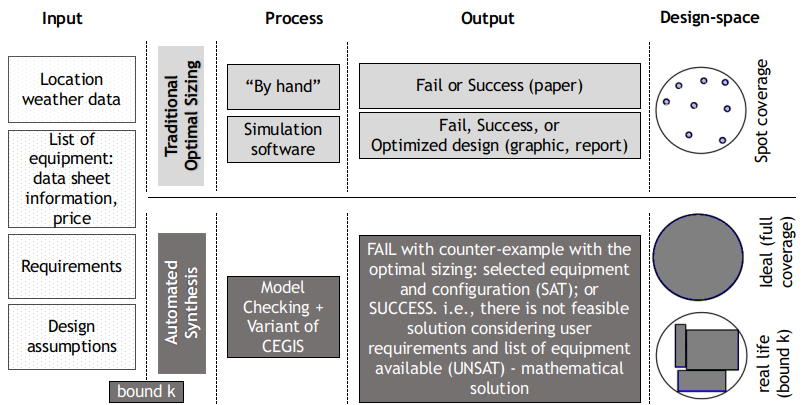
\includegraphics[width=1.0\textwidth]{optimalsizingprocess2g}
\centering
\caption{Comparison of optimal sizing methods}
\label{fig:optimization}
\end{figure}
 
\subsection{A Variant of CEGIS} 

Figure~\ref{CEGISalt} illustrates a variant of CEGIS, previously presented in Section ~\ref{sec:ProgramSynthesis}, Fig.~\ref{Counter-Example-Guided-Inductive-Synthesis}. This variant was created during the research for this thesis and will be detailed in this Section.

\begin{figure}[h]
	\centering
	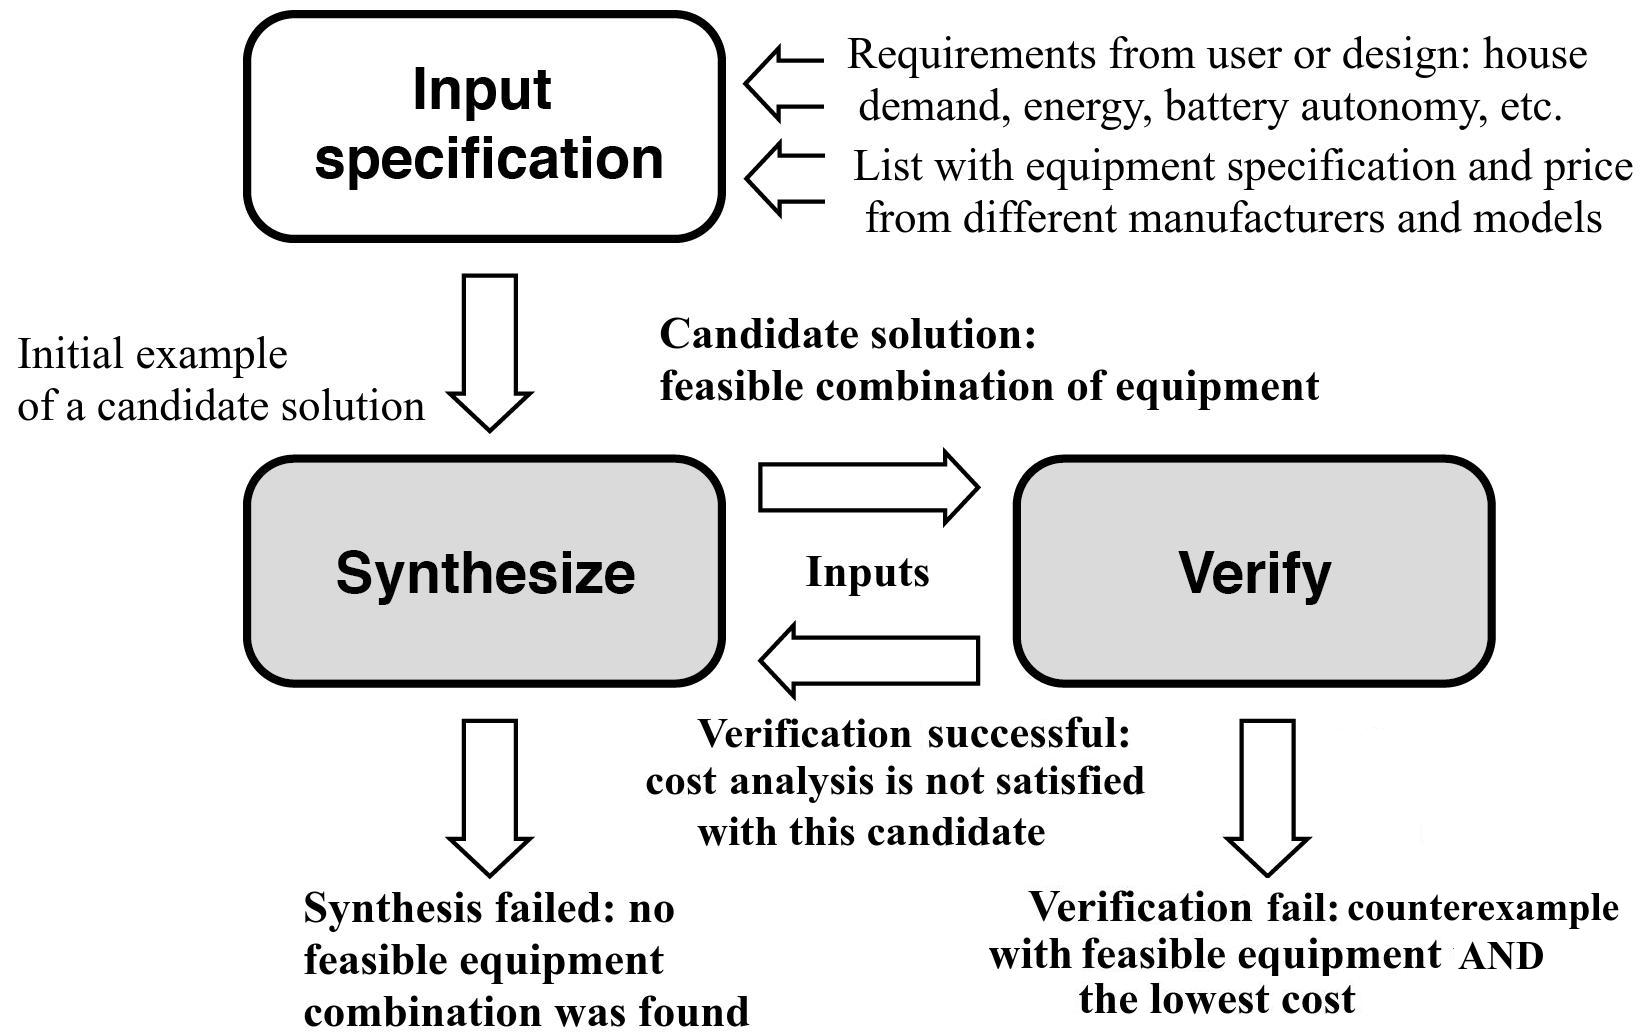
\includegraphics[width=0.75\columnwidth]{fig2_rev2.jpg}
	\caption{CEGIS applied to PV system sizing.}
	\label{CEGISalt}
\end{figure}

Examples of specification used by the proposed method include solar insolation (site dependent), house power demand, house  energy consumption, estimated load curve, AC voltage, and battery autonomy; we also provide a list of equipment specifications and prices from different manufacturers and models. Design assumptions are considered additional project specifications. The assumptions underlying optimal sizing are listed in Section~\ref{sec:OptAssumptions}.

The variant CEGIS used in the proposed approach differs in four specific aspects from the traditional CEGIS described in Figure ~\ref{Counter-Example-Guided-Inductive-Synthesis}: 

\begin{itemize}
\item There is no test vector and every candidate is generated during the run-time in the {\sc Synthesize} phase and sent to the {\sc Verify} phase; 
\item If the {\sc Verify} phase is unsuccessful, a new candidate is generated by {\sc Synthesize} 
\item The lower bound of the {\sc Verify} phase is incremented to search for the lowest cost; 
\item As a result, there is no refinement from the {\sc Verify} phase back to the {\sc Synthesize} phase, i.e. a new counterexample is not added to the {\sc input} set since a failure during the {\sc Verify} phase will only discard a given candidate that could be viable in the next iteration with a new lower bound.
\end{itemize}

Program synthesis engines that implement the CEGIS approach~\cite{sketch} can automatically produce solutions for a large variety of specifications; here we have used symbolic software verifiers based on SMT solvers.

Algorithm~\ref{alg:opt-algorithm} describes our pseudo-code to synthesize stand-alone PV systems using symbolic model checking. The analytical method of optimization was adopted, with LCC economic analysis and power reliability based on critical period criteria.

 \begin{algorithm}
 \caption{Synthesis algorithm}
 \begin{algorithmic}[1]
 \renewcommand{\algorithmicrequire}{\textbf{Input:}}
 \renewcommand{\algorithmicensure}{\textbf{Output:}}
  \REQUIRE weather data (temperature, solar irradiance), list of equipment (data sheet and price information), design requirements (load curve, peak demand, output voltage, battery autonomy), design assumptions (battery state of charge, criteria and objectives for technical and cost analysis)
 \ENSURE FAIL with counterexample showing the optimal sizing; SUCCESS, saying that the project has no feasible solution considering the requirements and the list of equipment available
  \STATE Initialize variables \\
  \STATE Declare list of PV panels, controllers, batteries, and inverters data and cost \\
%  \STATE Declare list of controllers data and cost \\
%  \STATE Declare list of batteries data and cost \\
%  \STATE Declare list of inverters data and cost \\
  \STATE Declare the maximum possible cost $MaxCost$  \\
  \STATE Declare power demand, power peak, energy consumption \\
  \STATE Declare battery autonomy, depth of discharge, AC voltage \\
  \FOR {$HintCost=0$ to $MaxCost$}
 	\STATE Declare non-deterministic variable to select PV Panel from list \\
 	\STATE Declare non-deterministic variable to select Controller from list \\
 	\STATE Declare non-deterministic variable to select Battery from list \\
 	\STATE Declare non-deterministic variable to select Inverter from list \\ 	
 	\STATE Calculate $E_{corrected}, \, E_{p} $ \\
	\STATE Calculate $N_{TPmin}, \, N_{PSmin}, N_{PPmin} $ \\
 	\STATE Calculate $C_{bank}$ \\
	\STATE Calculate $N_{BS}min, \, N_{BP}min, \, N_{B}total$ \\
	\STATE Requirement enforced by \textbf{assume}$(V_{c})$ \\
 	\STATE Calculate $I_{sc,amb}$ \\
 	\STATE Calculate $I_{c,min}$ \\
 	\STATE Requirement enforced by \textbf{assume}$(I_{c} \wedge V_{in}DC \wedge V_{out}AC)$ \\
%	\STATE Requirement enforced by \textbf{assume}$(V_{in}DC \wedge V_{out}AC )$ \\
%	\STATE Requirement enforced by \textbf{assume}$(V_{out}AC)$ \\
	\STATE Requirement enforced by \textbf{assume}$(Demand \wedge P_{surge})$ \\
%	\STATE Requirement enforced by \textbf{assume}$(P_{surge})$ \\
	\STATE non-deterministic variables hold feasible equipment and cost  \\
	\STATE $F_{obj} \leftarrow  N_{TP}*Panel_{Cost} \, + \, N_{TB}*Battery_{Cost} \, + Controller_{Cost} \, + \, Inverter_{Cost} \, + \, Installation_{Cost} \, + \, batrep_{Cost} \, + \, PWO\&M_{Cost}$ \\
	\STATE Violation check with \textbf{assert}$(F_{obj} > HintCost)$ \\
  \ENDFOR
 \RETURN $(\,)$ 
 \end{algorithmic} 
 \label{alg:opt-algorithm}
 \end{algorithm}

Our synthesis algorithm will synthesize constant values; 
it starts with the input of the manufacturer's data and prices of PV panels, batteries, charge controllers and inverters (line $2$). After that, we define user requirements, i.e. house requirements and design definitions, from lines $4$ and $5$. 

The \textit{for}-loop started at line $6$ controls the lowest cost of the PV solution. In particular, it starts with cost $0$ and stops only when the algorithm finds a feasible solution in which the cost breaks the $assertion$ stated in line $22$; if that happens, then our algorithm has found an optimal solution, thereby stating that the {\sc Verify} phase reached a satisfiable condition (\textit{SAT}). The $MaxCost$ value at line $6$ is just a very high value inserted as a limit to the \textit{for}-loop, that will never be reached because the optimal solution will be found first.

Our synthesis algorithm uses non-deterministic variables to choose one specific constant from a given list of PV panels, controllers, batteries and inverters (lines $7$ to $10$). This procedure ensures that our synthesis engine checks all combinations of items from each equipment, and combines them to assemble a viable (candidate) PV solution, which meets user requirements.

Next, we use Eq.~\eqref{eq:Ecorrected}, Eq.~\eqref{eq:Ep}, Eq.~\eqref{eq:NTPmin}, Eq.~\eqref{eq:NPSmin}, Eq.~\eqref{eq:NPPmin}, Eq.~\eqref{eq:Cbank}, Eq.~\eqref{eq:Nbtotal}, Eq.~\eqref{eq:iscamb} and Eq.~\eqref{eq:icmin} to calculate the sizing variables (lines $11$ to $17$). The directive \textit{assume} (lines $15$, $18$ and $19$) 
ensures compatibility of the items chosen from the list of equipment: the {\sc Verify} phase uses only items (among all the possible ones) that satisfy the statements of Lines $15$, $18$ and $19$. Line $15$ is specific to the charge controller voltage check. Line $18$ checks the inverter check $I_{c}$, the charge controller DC input voltage $V_{in}DC$, and charge controller AC output voltage $V_{in}DC$ check. Line $19$ ensures the power demand and the surge power of the inverter.
Therefore, our synthesis algorithm reaches line $20$ with one feasible solution, and the cost of that solution is calculated in $F_{obj}$ (line $21$). This cost is the equivalent to ~\ref{eq:LCC}, as described in Section ~\ref{sec:optcriteria}.

If our algorithm does not find a feasible solution among the item of equipment that were provided for our {\sc Synthesize} phase,  then the result is unsatisfiable (\textit{UNSAT}), i.e. the program finishes without finding a solution, indicating that it was not possible to combine the specific items of equipment in order to create a feasible solution. 

The main challenge for the {\sc Synthesize} phase is to find a feasible candidate solution for the constraints and user requirements. The challenge for the {\sc Verify} phase is to find the lowest acquisition cost from a list of equipment and components provided by the {\sc Synthesize} phase. 

Note that the process described here is completely automated and that a validation is performed by our {\sc Verify} phase to ensure that the approach is sound.

\subsection{Optimization Premises and Assumptions}
\label{sec:OptAssumptions}
%%%%%%%%%%%%%%%%%%%%%%%%%%%%%%%

This section contains premises and assumptions underlying the optimal sizing method, in relation to automated synthesis and simulation software.

In line $2$ of Algorithm~\ref{alg:opt-algorithm}, the synthesis engine is provided with a list of forty items of equipment from ten different manufacturers in order to allow the engine to choose from among all items of PV sizing. The necessary technical information was collected from data sheet of each item. In addition, the price of each item was obtained from available market quotation, in US dollars. All the other currencies were converted to US dollars equivalents at the exchange rate of the day.

With respect to power reliability, the critical period solar energy method will be used~\cite{Pinho}, as described in Section~\ref{sec:sizing}. The usual way is to use loss of load probability (LOLP) or loss of power supply probability (LPSP). However, due to the fact that in this study we are considering neither site characteristics nor load changes over time, which demand historical data, the reliability analysis will be developed only by the critical period method of PV sizing.

Financial analysis details:
\begin{itemize}
	\item LCC lifetime considered: $20$ years;
	\item Installation costs: these include delivery to the isolated community and the actual installation costs: $5$\% of total cost~\cite{Agrener2013};
	\item Value of the discount rate or interest rate: $10$\%, a good rate, considering financial investments in developing countries;
	\item Annual operation and maintenance costs: based on past PV projects of similar size in the Brazilian Amazon, the sum of US\$ 289.64~\cite{Agrener2013} will be adopted. This cost includes battery replacement based on a lifetime of $4$ years for lead-acid batteries, plus inverters and controller replacement (every $10$ years). This means that there will be three battery bank and one inverter-controller replacement during the LCC analysis.
\end{itemize}

The PV system optimization technique adopted here is the intuitive method, since the average daily value of solar irradiance is used in the mathematical model, without considering battery state of charge, or even the random nature of solar irradiation and meteorological conditions. Therefore, all the computational effort will be concentrated on our automated synthesis algorithm.

With regard to batteries, the voltage of the system (DC bus) is set at $24$ V DC (but this can be adjusted to $12$ or $48$ V in the code).

HOMER Pro details:

\begin{itemize}
	\item HOMER Pro does not provide for the LCC cost in its reports. However, it has NPC and LCOE. For this reason, NPC was used to obtain LCC in order to allow the comparison among tools;
	\item The optimization analysis of HOMER Pro permits the definition of a load curve and temperature on the basis of data collected automatically from online databases. However, in order to enable a correct comparison, the curve load and the temperature were defined exactly the same as automated synthesis tools;
	\item Battery autonomy is not a parameter that the user can set when using HOMER Pro. The tool will always meet the user requirement, i.e. the load curve, $365$ days a year;
	\item HOMER Pro does not have an item of equipment explicitly labeled charge controller. It uses a controller resource that can perform in two different ways, depending on optimization choice or user choice: load following or cycle charging~\cite{HOMER}. During the tests  'load following' controller was chosen: it produces only enough power to meet the demand~\cite{HOMER};
	\item A 5\% of capacity shortage was assumed, equivalent to 95\%  availability of the PV system. By definition, availability is the percentage of time during which a power system is capable of meeting the load requirements~\cite{Khatib2014}. For critical loads, 99\% is considered acceptable, while in an ordinary residential electrical load, 95\% is considered acceptable;
	\item A string of two batteries was assumed in order to match the system voltage of $24$ V DC used by the automated synthesis tool;
	\item The premise adopted when using HOMER Pro was that the user does not know the optimal solution, and that in order to obtain this solution it is necessary to include (at the design phase of the tool) generic PV and battery modules that HOMER Pro will search for the optimized power of each component. With that in mind, a generic flat plate PV of $1$ kW was included and generic lead-acid batteries of $1$ kW also (and with capacity of $83.4$ Ah in accordance with HOMER Pro modeling). HOMER, during run-time, decides the size in kW of each module, based on feasibility and lower cost.	
\end{itemize}

\section{General Assumptions}

The general assumptions for the scientific method of automated synthesis are the same presented in Section~\ref{sec:assumptions}, with respect to the code in ANSI-C, to the bound $k$, to the simulation tool comparison, and to the battery state of charge.

%---------------------------------------------------------------------------
\section{Description of the Case Studies} 
%---------------------------------------------------------------------------

The proposed synthesis approach was evaluated in  seven stand-alone PV system case studies: 

\begin{itemize}
\item Case Study 1: Power peak: 342 W, power surge: 342 W, energy consumption: 3,900 Wh/day, battery autonomy: 48 h;
\item Case Study 2: Power peak: 814 W, power surge: 980 W, energy consumption: 4,880 Wh/day, battery autonomy: 48 h;
\item Case Study 3: Power peak: 815 W, power surge: 980 W, energy consumption: 4,880 Wh/day, battery autonomy: 12 h;
\item Case Study 4: Power peak: 253 W, power surge: 722 W, energy consumption: 3,600 Wh/day, battery autonomy: 48 h;
\item Case Study 5: Power peak: 263 W, power surge: 732 W, energy consumption: 2,500 Wh/day, battery autonomy: 48 h;
\item Case Study 6: Power peak: 322 W, power surge: 896 W, energy consumption: 4,300 Wh/day, battery autonomy: 48 h;
\item Case Study 7: Power peak: 1,586 W, power surge: 2,900 W, energy consumtion: 14,000 Wh/day, battery autonomy: 48h.
\end{itemize}

These case studies were defined based on the usual electrical load found in riverside communities in the State of Amazonas,  Brazil~\cite{TrindadeCordeiro19, Agrener2013}, with the exception of case 7, that was idealized as a small town solution to support a few lamps and a 12 kBTUs air-conditioner.

%---------------------------------------------------------------------------
\section{Objectives and Setup}
\label{sec:synthesissetup} 
%---------------------------------------------------------------------------

The evaluation aims to answer two experimental questions: 

\begin{enumerate}

\item[EQ1] \textbf{(soundness)} does the proposed automated synthesis approach provide correct results?

\item[EQ2] \textbf{(performance)} how do the software verifiers compare to each other?

\end{enumerate}

All experiments regarding the verification tools were conducted 
on an otherwise idle Intel Xeon CPU E5-4617 ($8$-cores) with 
$2.90$ GHz and $64$ GB RAM, running Ubuntu $16.04$ LTS $64$-bits. 
For HOMER Pro, an Intel Core i5-$4210$ ($4$-cores) was used, 
with $1.7$ GHz and $4$ GB RAM, running Windows 10. 
The experiments were conducted with a predefined time-out of $240$ minutes.

Three start-of-the-art verification tools, CBMC\footnote{Command-line: \$ cbmc -\phantom{}-unwind 100 filename.c -\phantom{}-trace} version 5.11 with MiniSat 2.2.1~\cite{Kroening}, ESBMC\footnote{Command-line: \$ esbmc filename.c -\phantom{}-no-bounds-check -\phantom{}-no-pointer-check -\phantom{}-unwind 100 -\phantom{}-boolector} version 6.0.0 with the  Boolector 3.0.1 solver~\cite{Brummayer}, %UAutomizer\footnote{Command-line: \$ ./Ultimate -tc config/AutomizerReach.xml -s config/svcomp-Reach-32bit-Automizer\_Default.epf -i filename.c -\phantom{}-traceabstraction.limit.analysis.time 900 -\phantom{}-traceabstraction.stop.after.first.violation.was.found false -\phantom{}-cacsl2boogietranslator.overapproximate.operations.on.floating.types false -\phantom{}- cacsl2boogietranslator.assume.nondeterminstic.values.are.in.range false -\phantom{}-rcfgbuilder.add.additional.assume.for.each.assert true -\phantom{}-rcfgbuilder.simplify.code.blocks true -\phantom{}-rcfgbuilder.size.of.a.code.block LoopFreeBlock}, 
and CPAchecker\footnote{Command-line: \$ scripts/cpa.sh -heap 64000m -config config/bmc-incremental.properties -spec config/specification/sv-comp-reachability.spc filename.c} version 1.8 with MathSAT 5.5.3~\cite{mathsat5}, were used as verification engines to compare the proposed approach effectiveness and efficiency. Note that ``incremental'' ESBMC with the SMT solver Z3 version 4.7.1~\cite{DeMoura} was tried\footnote{Command-line: \$ esbmc filename.c -\phantom{}-no-bounds-check -\phantom{}-no-pointer-check -\phantom{}-unwind 100 -\phantom{}-smt-during-symex -\phantom{}-smt-symex-guard -\phantom{}-z3} as an alternative to use less computing memory. The Simulation tool HOMER Pro version $3.13.1$ was used for comparative purposes.

%---------------------------------------------------------------------------
\section{Experimental Results}  
\label{sec:synthesisresults}
%---------------------------------------------------------------------------

The results are presented at Table~\ref{tab1}. 

\begin{table}
\caption{Case studies and results: optimization of stand-alone PV systems.}\label{tab1}
\begin{scriptsize}
\begin{tabular}{|c|c|c|c|c|}
\hline
\hline
Tools & \makecell{CBMC 5.11 \\(MiniSat 2.2.1)}& \makecell{ESBMC 6.0.0 \\(Boolector 3.0.1 /\\Z3 4.7.1)}& \makecell{CPAchecker 1.8\\(MathSAT 5.5.3)}& HOMER Pro 3.13.1\\
\hline
\hline
Specification & Result & Result & Result & Result \\
\hline
\makecell{\textbf{Case Study 1}\\Peak:342W\\Surge:342W \\E:3,900Wh/day\\Autonomy:48h} & OM & TO / IF & \makecell{SAT (172.03 min) \\NTP:1$\times$340W (1S)\\NBT:8$\times$105Ah (2S-4P)\\Controller 15A/75V\\Inverter 700W/48V\\LCC: US\$ 7,790.53} & \makecell{(Time: 0.33 min)\\2.53 kW of PV\\NBT:12$\times$83.4Ah (2S-6P)\\0.351kW inverter\\LCC: US\$ 7,808.04}\\
\hline
\makecell{\textbf{Case Study 2}\\Peak:814W\\Surge:980W\\E:4,880Wh/day\\Autonomy:48h} & OM & TO / IF & \makecell {SAT (228.7 min) \\NTP:2$\times$330W (2S)\\NBT:10$\times$105Ah (2S-5P)\\Controller 20A/100V DC\\Inverter 1,200W/24V \\LCC: US\$ 8,335.90} & \makecell{(Time: 0.18 min)\\3.71 kW of PV\\NBT:20$\times$83.4Ah (2S-10P)\\0.817kW inverter\\LCC: US\$ 12,861.75} \\
\hline
\makecell{\textbf{Case Study 3}\\Peak:815W\\Surge:980W\\E:4,880Wh/day\\Autonomy:12h} & OM & TO / IF & \makecell {SAT (166.13 min) \\NTP:4$\times$150W (4S)\\NBT:4$\times$80Ah (2S-2P)\\Controller 15A/100V DC\\Inverter 1,200W/24V \\LCC: US\$ 7,306.27} & Not possible \\
\hline
\makecell{\textbf{Case Study 4}\\Peak:253W\\Surge:722W\\E:3,600Wh/day\\Autonomy:48h} & OM & TO / IF & \makecell {SAT (143.71 min) \\NTP:4$\times$150W (4S)\\NBT:10$\times$80Ah (2S-5P)\\Controller 15A/75V\\Inverter 750W/24V \\LCC: US\$ 7,816.31} & \makecell{(Time: 0.23 min)\\2.42 kW of PV\\NBT:12$\times$83.4Ah (2S-6P)\\0.254kW inverter\\LCC: US\$ 7,677.95}\\
\hline
\makecell{\textbf{Case Study 5}\\Peak:263W\\Surge:732W\\E:2,500Wh/day\\Autonomy:48h} & OM & TO / IF & \makecell {SAT (134.93 min) \\NTP:1$\times$340W (1S)\\NBT:6$\times$105Ah (2S-3P)\\Controller 15A/75V\\Inverter 400W/24V \\LCC: US\$ 7,252.14} & \makecell{(Time: 0.18 min)\\1.59 kW of PV\\NBT:10$\times$83.4Ah (2S-5P)\\0.268kW inverter\\LCC: US\$ 6,175.57} \\
\hline
\makecell{\textbf{Case Study 6}\\Peak:322W\\Surge:896W\\E:4,300Wh/day\\Autonomy:48h} & OM & TO / IF & \makecell {SAT (235.75 min) \\NTP:2$\times$200W (2S)\\NBT:10$\times$105Ah (2S-5P)\\Controller 15A/75V\\Inverter 400W/24V \\LCC: US\$ 8,287.23} & \makecell{(Time: 0.22 min)\\3.15 kW of PV\\NBT:14$\times$83.4Ah (2S-7P)\\0.328kW inverter\\LCC: US\$ 9,112.45} \\
\hline
\makecell{\textbf{Case Study 7}\\Peak:1,586W\\Surge:2,900W\\E:14,000Wh/day\\Autonomy:48h} & OM & TO / IF & TO & \makecell{(Time: 0.20 min)\\12.5 kW of PV\\NBT:66$\times$83.4Ah (2S-33P)\\1.60kW inverter\\LCC: US\$ 41,878.11} \\
\hline
\hline
\end{tabular}
\\Legend: OM = out of memory; TO = time out; IF = internal failure, E = energy.
\end{scriptsize}
\end{table}

CPAchecker was able to synthesize optimal sizing in six 
out of the seven case studies (cases $1$ - $6$): the result was produced within the time limit, which varied from $134.71$ to $235.75$ minutes. Fig.~\ref{fig:CPAoptc1} illustrates the result of case 4 with the optimal sizing appearing on the left size as the integer $8$ for the solar panel (which is the model RSM36-6-150P from the manufacturer Risen), battery $0$ refers to the model 12MF80 of 80 Ah from Moura, charge controller $1$ refers to the model 15A-75V MPPT from Victron  Energy, and the inverter number $3$ refers to the model IP350-11 from Epever (750 W). The variables NTP, NPS, NPP, NPS, NBP, and NBTotal, also presented in the counterexample as well, shows the number of panels and batteries and how they are connected.

Only case study $7$ led to a \textit{time out} result in CPAchecker, i.e.  it was not solved within $240$ minutes. This is illustrated in Fig.~\ref{fig:cpaoptcase7}. However, this CPAchecker time-out limitation is removed, the verifier is able to solve the optimization in $44.97$ hours. The violation (SAT result) indicated in Table~\ref{tab1} 
is the $assert$ of line $22$ from Algorithm~\ref{alg:verification-algorithm}. %The results were tested by manual PV sizing and were sound (\textit{RQ1}). %, linking a feasible technical solution with the lowest cost possible, considering the equipment that were inputted to the code. 

\begin{figure}[h]
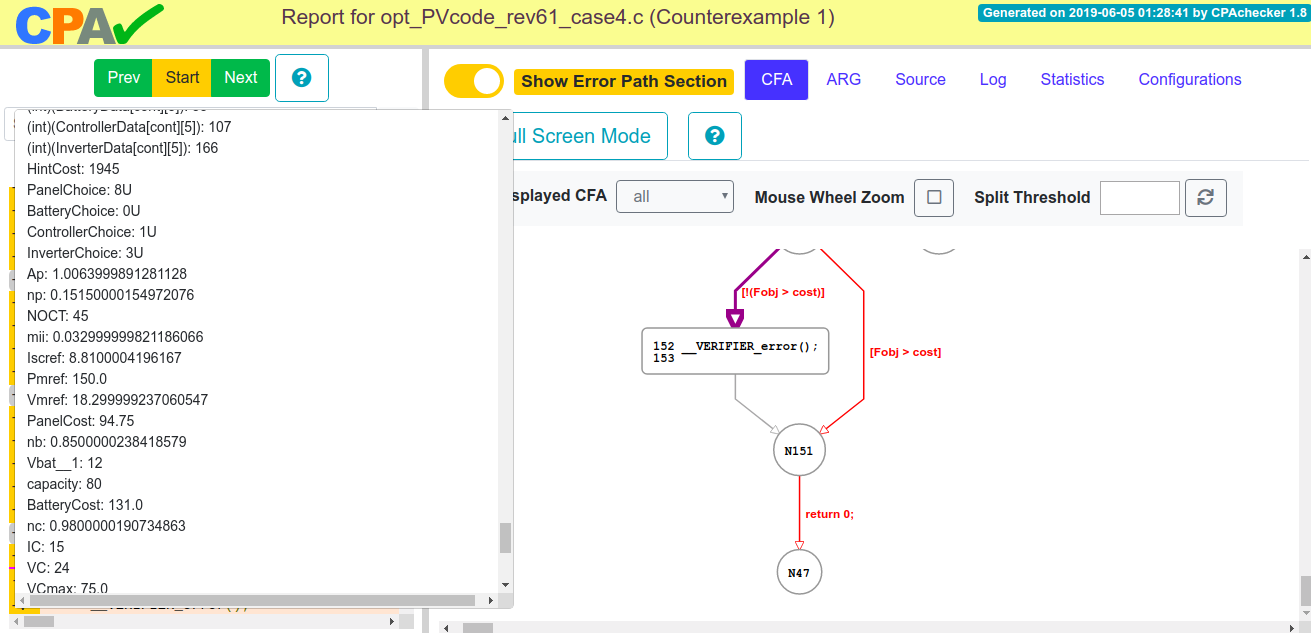
\includegraphics[width=1.0\textwidth]{CPA_opt_c4.png}
\centering
\caption{Counterexample generated by CPAchecker after validation of case 4 (file Counterexample.html).}
\label{fig:CPAoptc1}
\end{figure}

\begin{figure}[h]
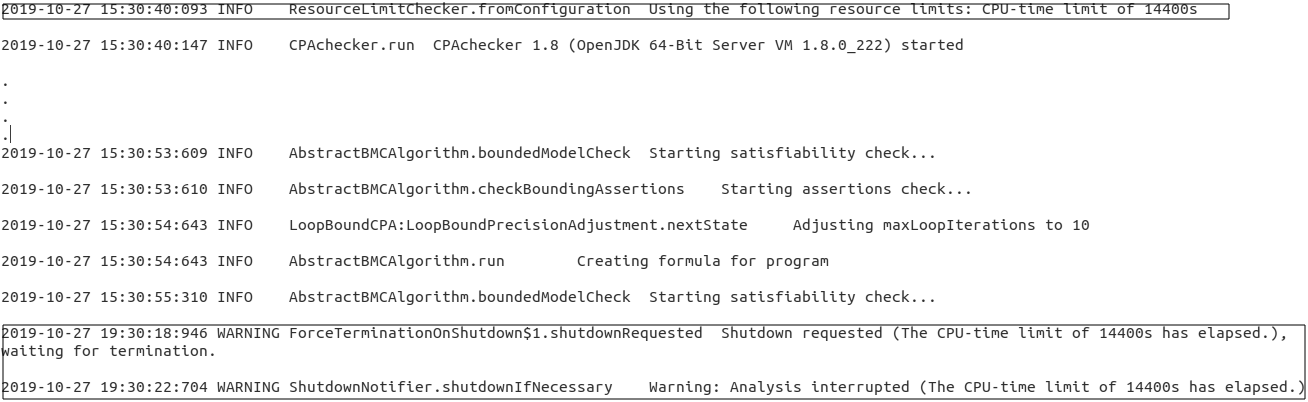
\includegraphics[width=1.0\textwidth]{CPAchecker_timeout_case7.png}
\centering
\caption{CPAchecker time out result for case 7 optimization (file CPALog.txt).}
\label{fig:cpaoptcase7}
\end{figure}

CBMC and ESBMC are unable to produce any conclusive result. \textit{Internal failure}, \textit{time out}, or \textit{out of memory} situations occurred; this partially answers the \textit{EQ2}. Note that the internal failure presented by ESBMC was a Z3 solver issue (a bug), which will require an updated version of ESBMC to fix. Similar to CPAchecker, if the \textit{time out} is removed from ESBMC with the SMT solver Boolector, then the verifier is able to obtain the automated synthesis in $73.18$ hours for case study $2$. CBMC, on the other hand,  could present some result only if the RAM memory of the system was expanded in order to avoid the out of memory issue.

HOMER Pro was able to evaluate six case studies (cases $1$, $2$, $4$, $5$, $6$, and $7$), and in under $30$ seconds, much faster than the proposed automated synthesis tool (cf.~\textit{EQ2}). Case study $3$ could not be simulated since HOMER Pro does not have the battery autonomy adjustment feature, i.e. the tool always tries to feed the given load with electricity $365$ days/year. 

Fig.~\ref{fig:homeroptc4} illustrates parts of the 9-page PDF report presented by HOMER Pro, specifically for case 4.

\begin{figure}[h]
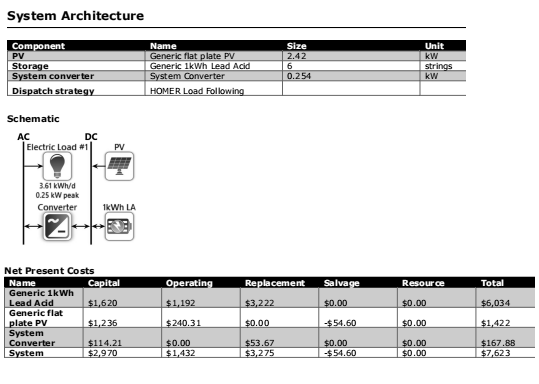
\includegraphics[width=0.8\textwidth]{homeroptc4.png}
\centering
\caption{Optimization report (partial) from HOMER Pro (case 4).}
\label{fig:homeroptc4}
\end{figure}

Certain other HOMER Pro drawbacks were also noted:

\begin{itemize}
\item System equipment does not include an explicit charge controller . HOMER Pro includes a controller automatically just to simulate the charge/discharge of batteries and to meet the load requirement; however, without costs or even with electrical characteristics such as maximum current and voltage, which are common during PV sizing;
\item HOMER Pro requires the inclusion of some battery specification to initiate optimization; however, it does not change the electrical specifications during simulation; the results presented are multiples of the original battery type suggested by the user. For example, it was started with a $83.4$ Ah lead-acid battery and during simulation, HOMER Pro did not try to use other capacities or types;
\item HOMER Pro does not present the optimal solution in terms of connections of PV panel arrays, just the total in terms of power, i.e. it presents neither the models and the power of each PV panel nor the total of panels in series or parallel.
\end{itemize}

%%%%%%%%%%%%%%%%%%%%%%%%%%%%%%%%%%%%%%%%%%%%%%%%%%%%%%%%%%%%%%%%%%%%
\subsection{Comparison Between Formal Synthesis and HOMER Pro}
%%%%%%%%%%%%%%%%%%%%%%%%%%%%%%%%%%%%%%%%%%%%%%%%%%%%%%%%%%%%%%%%%%%%

Comparing the results of the formal synthesis against those of CPAchecker and HOMER Pro, it was observed that most results are quite similar, 
in terms of technical solution and cost (cf. Table~\ref{tab1}). 

Particularly in the case of LCC, the cost was very close in cases $1$, $4$, $5$ and $6$, with differences varying from $0.23$\% to $17.4$\%. Even adopting the same price per kW for PV panels, inverters, and batteries, HOMER Pro does not use costs related to charge controllers, which were introduced into the CPAchecker modeling. The premise used in CPAchecker to adopt a fixed annual cost for operation and maintenance can produce some impact as well on this discrepancy; however, it is not significant since the annual cost is too small when compared to the resulting LCC value.

However, there exists a huge divergence in case study $2$, where the costs presented by HOMER Pro were $54$\% higher than the automated synthesis tool, probably because the operation and maintenance costs assumed by the automated synthesis tool were underestimated for that specific load. 

In general, the PV panels and battery bank were larger in HOMER Pro than with the formal synthesis approach, and that discrepancy is not easy to address without some real systems validation. The mathematical models are different and particular parameters can be tuned as well in each approach, and that can justify the difference, which was presented in all the case studies. As a comparison, consider case study $1$: the optimal solution provided by HOMER Pro requires $7$ $times$ more PV panels than the solution presented by the synthesis tool, and HOMER Pro does not show the arrangement of arrays (i.e. the number of series and parallel PV panels); the battery bank presented by HOMER Pro provides a capacity of $500.4$ Ah ($6 \times 83.4$), while the synthesis tool presented an optimal solution with a total capacity of $420$ Ah ($4 \times 105$). 

Comparing the optimization results with those the real-world, the author had four PV systems deployed and monitored since June $2018$ in a riverside community in State pf Amazonas, Brazil, with demands  similar to those of case studies $1$, $4$, $5$, and $6$, always with a $3$ $\times$ $325$ W ($3$S) panels and $4$ $\times$ $220$ Ah ($2$S-$2$P $= 440$ Ah) lead-acid batteries. These solutions are closer to the result presented by the proposed formal synthesis approach than that of HOMER Pro, thereby showing that the solution is sound, which answers \textit{EQ1}.

HOMER Pro suggests a value in kW for the inverters that is very close to the peak of every case study, and it is just a reference value and not a commercial value of the inverter employed. The proposed synthesis tool, however, presents inverters that are commercial and can be bought off-the-shelf. This is a clear advantage of the formal synthesis method.

As was reported in section~\ref{sec:synthesisresults}, HOMER Pro does not include charge controllers as an explicit item of equipment in its mathematical model; only the synthesis tool presents a commercial controller and includes it during the cost analysis. The formal synthesis method, therefore, presents more reliable results than HOMER Pro.

Case study $7$ was not solved by the synthesis tool within the time limit established during the experimental phase. Case study $3$ could not be simulated in HOMER Pro, because of its restriction on setting battery autonomy, thus leaving both without parameters to compare.

Summarizing, the synthesis tool is capable of presenting a solution which is far more detailed and closer to commercial conditions than the solution presented by HOMER Pro. In particular, the automated synthesis method can provide all the details of every component of a PV system solution, with complete electrical details from the manufacturer data sheet, including  the model of the component, nominal current and voltage. In this respect, even the name of the manufacturer can be cited (in Table~\ref{tab1} it was removed to avoid unauthorized advertising).
%used with the SMT incremental mode\footnote{Command-line: \$ esbmc filename.c -\phantom{}-no-bounds-check -\phantom{}-no-pointer-check -\phantom{}-unwind 100 -\phantom{}-smt-during-symex -\phantom{}-smt-symex-guard -\phantom{}-z3} enabled with the goal of reducing memory usage; we have also used the SMT solver Z3 version 4.7.1~\cite{DeMoura}.

%%%%%%%%%%%%%%%%%%%%%%%%%%%%%%%%%%%%%%%%%%
\section{Threats to validity}
%%%%%%%%%%%%%%%%%%%%%%%%%%%%%%%%%%%%%%%%%%

In this Section, a favorable assessment was made of the proposed formal synthesis method. Nevertheless, three threats to the validity of the experimental results were also identified, which can be further assessed and 
constitute future work: 

\begin{itemize}
\item ($1$) improvement to the power reliability analysis: inclusion of loss of load probability or loss of power supply probability, in order to increase the accuracy of the analysis; 
\item ($2$) the cost analysis is well tailored to Brazilian Amazon; however, a broad analysis of other isolated areas must be  performed in order to make the optimization general in terms of applicability; 
\item ($3$) deployment in the field of PV systems sized using the synthesized results in order to validate them.
\end{itemize}


\section{Conclusion}

In this Chapter we showed in detail how the state-of-the-art computer science method of automated synthesis has been adapted to use in stand-alone solar PV systems in order to obtain optimal project sizing. Moreover, it was possible to illustrate how the proposed method compares with the traditional use of a simulation tool for the same purpose.

Detailed diagrams, flowcharts and algorithms with pseudo-code were presented as support for the proposed work and to aid understanding. Also listed, were the assumptions underlying the automated verification and simulation software. 

Comparison of verifiers with the proposed automated synthesis using model checking was made, in order to obtain the optimal sizing of stand-alone solar PV systems, which showed that CPAchecker had the best overall performance. CBMC and ESBMC were not conclusive for all the cases, reaching the \textit{time out} stipulated ($240$ minutes) or being \textit{out of memory}. CPAchecker was unable to present a conclusive result only in case $7$ (\textit{time out}).

A comparison with a specialized simulation tool was also made, however only $5$ case studies (case $1$, case $2$, case $4$, case $5$, and case $6$) compared to the presented result. Some limitations of the simulation tool, mainly related to not allowing battery autonomy setup, and the $time-out$ or $out of memory$ messages presented by the verifiers, restricted the comparison between the automated verification tools and the simulation tools. However, when the comparison was possible, it was noticeable that the LCC came very close, and that HOMER Pro overestimated the sizing.

Based on the fact that mostly case studies were deployed in the field (case $1$, case $4$, case $5$, and case $6$), with regular visits to conduct interviews with the residents, and consult the monitoring system in those houses, it was possible to compare the computer assisted results with the real-world employment of stand-alone solar PV systems. The final conclusion was that the proposed tool is sound, with an acceptable performance, and a higher quality output.